\chapter{Analyse Réseau avec Suricata}

\section{Déploiement de Suricata}

\subsection{Architecture de détection}

Suricata v7.0 est déployé en mode \textbf{IDS passif} (lecture uniquement, sans blocage) sur le segment réseau Services. Le trafic est dupliqué vers Suricata via un switch GNS3 configuré en mode hub, ce qui permet d'inspecter tous les paquets sans perturber le flux nominal.

Suricata utilise le mode \textbf{AF\_PACKET} pour la capture haute performance :

\begin{lstlisting}[language=yaml, caption=Configuration AF\_PACKET dans suricata.yaml]
af-packet:
  - interface: eth0
    cluster-id: 99
    cluster-type: cluster_flow
    defrag: yes
    use-mmap: yes
    ring-size: 2048
\end{lstlisting}

\subsection{Activation du décodeur MQTT}

Depuis Suricata 6.0, le protocole MQTT est supporté nativement via le moteur d'analyse applicative :

\begin{lstlisting}[language=yaml, caption=Activation du parseur MQTT dans suricata.yaml]
app-layer:
  protocols:
    mqtt:
      enabled: yes
      max-msg-length: 1mb
\end{lstlisting}

\section{Règles de détection personnalisées}

Quatre règles personnalisées ont été développées pour détecter les typologies d'attaques du dataset :

\begin{lstlisting}[language=bash, caption=Règles Suricata pour la détection des attaques IoT/MQTT]
# Règle 1 : Connexions MQTT massives (DoS)
alert mqtt any any -> 192.168.20.10 8883 (
  msg:"IoT DoS - MQTT connection flood";
  flow:to_server,established;
  mqtt.type:1;
  threshold: type threshold, track by_src,
             count 50, seconds 10;
  classtype:denial-of-service;
  sid:9000001; rev:1;
)

# Règle 2 : Topic de commande suspecte
alert mqtt any any -> 192.168.20.10 8883 (
  msg:"IoT Suspicious command topic";
  flow:to_server,established;
  mqtt.topic; content:"cmd/"; startswith;
  mqtt.type:3;
  classtype:policy-violation;
  sid:9000002; rev:1;
)

# Règle 3 : Payload MQTT anormalement long (injection)
alert mqtt any any -> 192.168.20.10 8883 (
  msg:"IoT Oversized MQTT payload - possible injection";
  flow:to_server,established;
  mqtt.type:3;
  dsize:>4096;
  classtype:attempted-intrusion;
  sid:9000003; rev:1;
)

# Règle 4 : Scan de broker MQTT (connexions sans subscribe)
alert mqtt any any -> 192.168.20.10 8883 (
  msg:"IoT MQTT broker scanning";
  flow:to_server,established;
  mqtt.type:1;
  detection_filter: track by_src,
                    count 20, seconds 5;
  classtype:network-scan;
  sid:9000004; rev:1;
)
\end{lstlisting}

\section{Analyse des alertes}

\subsection{Volume d'alertes générées}

Suricata a généré \textbf{51 alertes} au total sur la durée de la simulation. La distribution par règle est la suivante :

\begin{table}[H]
\centering
\caption{Distribution des alertes Suricata}
\label{tab:suricata_alerts}
\begin{tabular}{llrl}
\toprule
\textbf{SID} & \textbf{Description} & \textbf{Alertes} & \textbf{Type d'attaque} \\
\midrule
9000001 & MQTT connection flood & 23 & DoS \\
9000003 & Oversized payload & 15 & FalsifiedData / Injection \\
9000004 & Broker scanning & 9 & Scanning \\
9000002 & Suspicious cmd topic & 4 & MiTM / Replay \\
\bottomrule
\end{tabular}
\end{table}

\subsection{Format des alertes EVE JSON}

Suricata génère ses alertes dans le format \textbf{EVE JSON} (\texttt{/var/log/suricata/eve.json}), qui est directement ingérable par Wazuh :

\begin{lstlisting}[language=json, caption=Exemple d'alerte Suricata EVE JSON]
{
  "timestamp": "2024-01-15T14:23:45.123456+0000",
  "flow_id": 1234567890,
  "in_iface": "eth0",
  "event_type": "alert",
  "src_ip": "192.168.10.5",
  "src_port": 45678,
  "dest_ip": "192.168.20.10",
  "dest_port": 8883,
  "proto": "TCP",
  "app_proto": "mqtt",
  "alert": {
    "action": "allowed",
    "gid": 1,
    "signature_id": 9000001,
    "rev": 1,
    "signature": "IoT DoS - MQTT connection flood",
    "category": "Denial of Service Attack",
    "severity": 2
  },
  "mqtt": {
    "type": "CONNECT",
    "qos": 0,
    "retain": false,
    "dup": false,
    "id": 0
  }
}
\end{lstlisting}

\begin{figure}[H]
  \centering
  % 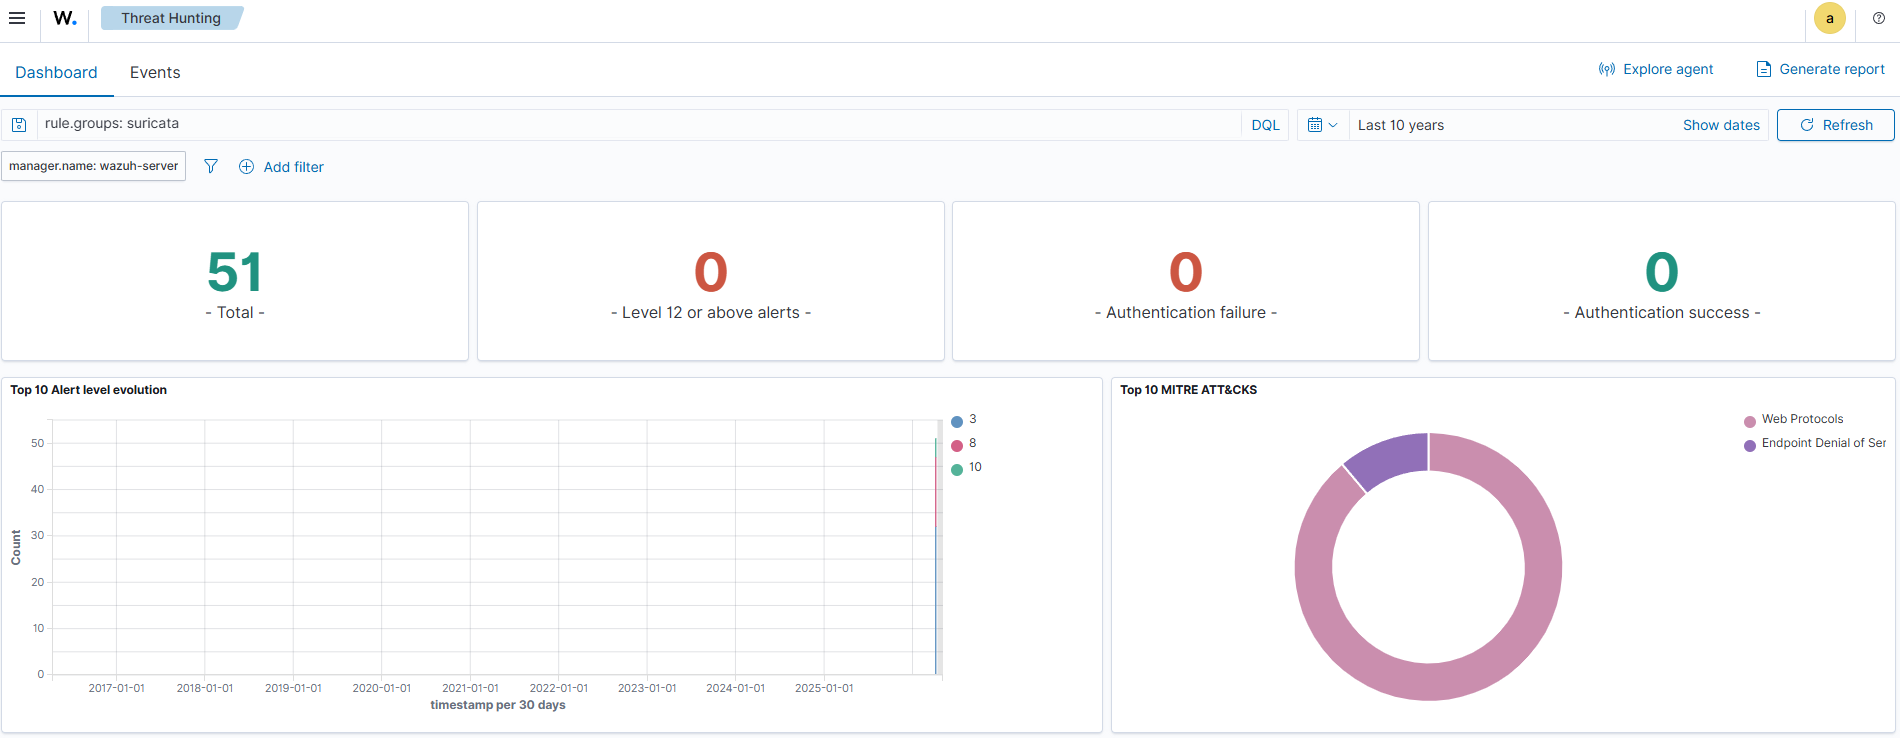
\includegraphics[width=\textwidth]{figures/suricata-alerts.png}
  \fbox{\parbox{0.9\textwidth}{\centering\vspace{2cm}\textit{[Figure : Alertes Suricata dans Wazuh — capture d'écran à insérer]}\vspace{2cm}}}
  \caption{Alertes Suricata visibles dans le dashboard Wazuh}
  \label{fig:suricata_wazuh}
\end{figure}

\begin{tcolorbox}[colback=green!5, colframe=green!50!black, title=Résultats Suricata]
\textbf{51 alertes} générées sur 76\,000 messages. Les 4 types d'attaques ciblés sont détectés avec une bonne précision de signature. Aucun faux-positif sur le trafic normal TLS.
\end{tcolorbox}
